\documentclass[class=article, crop=false]{standalone}
\usepackage[margin=1in]{geometry}
\usepackage[linesnumbered,ruled,vlined]{algorithm2e}
\usepackage{amsfonts}
\usepackage{amsmath}
\usepackage{amssymb}
\usepackage{amsthm}
\usepackage{enumitem}
\usepackage{fancyhdr}
\usepackage{hyperref}
\usepackage{minted}
\usepackage{multicol}
\usepackage{pdfpages}
\usepackage{standalone}
\usepackage[many]{tcolorbox}
\usepackage{tikz-cd}
\usepackage{transparent}
\usepackage{xcolor}
% \tcbuselibrary{minted}

\author{Nathan Solomon}

\newcommand{\fig}[1]{
    \begin{center}
        \includegraphics[width=\textwidth]{#1}
    \end{center}
}

% Math commands
\renewcommand{\d}{\mathrm{d}}
\DeclareMathOperator{\id}{id}
\DeclareMathOperator{\im}{im}
\DeclareMathOperator{\proj}{proj}
\DeclareMathOperator{\Span}{span}
\DeclareMathOperator{\Tr}{Tr}
\DeclareMathOperator{\tr}{tr}
\DeclareMathOperator{\ad}{ad}
\DeclareMathOperator{\ord}{ord}
%%%%%%%%%%%%%%% \DeclareMathOperator{\sgn}{sgn}
\DeclareMathOperator{\Aut}{Aut}
\DeclareMathOperator{\Inn}{Inn}
\DeclareMathOperator{\Out}{Out}
\DeclareMathOperator{\stab}{stab}

\newcommand{\N}{\ensuremath{\mathbb{N}}}
\newcommand{\Z}{\ensuremath{\mathbb{Z}}}
\newcommand{\Q}{\ensuremath{\mathbb{Q}}}
\newcommand{\R}{\ensuremath{\mathbb{R}}}
\newcommand{\C}{\ensuremath{\mathbb{C}}}
\renewcommand{\H}{\ensuremath{\mathbb{H}}}
\newcommand{\F}{\ensuremath{\mathbb{F}}}

\newcommand{\E}{\ensuremath{\mathbb{E}}}
\renewcommand{\P}{\ensuremath{\mathbb{P}}}

\newcommand{\es}{\ensuremath{\varnothing}}
\newcommand{\inv}{\ensuremath{^{-1}}}
\newcommand{\eps}{\ensuremath{\varepsilon}}
\newcommand{\del}{\ensuremath{\partial}}
\renewcommand{\a}{\ensuremath{\alpha}}

\newcommand{\abs}[1]{\ensuremath{\left\lvert #1 \right\rvert}}
\newcommand{\norm}[1]{\ensuremath{\left\lVert #1\right\rVert}}
\newcommand{\mean}[1]{\ensuremath{\left\langle #1 \right\rangle}}
\newcommand{\floor}[1]{\ensuremath{\left\lfloor #1 \right\rfloor}}
\newcommand{\ceil}[1]{\ensuremath{\left\lceil #1 \right\rceil}}
\newcommand{\bra}[1]{\ensuremath{\left\langle #1 \right\rvert}}
\newcommand{\ket}[1]{\ensuremath{\left\lvert #1 \right\rangle}}
\newcommand{\braket}[2]{\ensuremath{\left.\left\langle #1\right\vert #2 \right\rangle}}

\newcommand{\catname}[1]{{\normalfont\textbf{#1}}}

\newcommand{\up}{\ensuremath{\uparrow}}
\newcommand{\down}{\ensuremath{\downarrow}}

% Custom environments
\newtheorem{thm}{Theorem}[section]

\definecolor{probBackgroundColor}{RGB}{250,240,240}
\definecolor{probAccentColor}{RGB}{140,40,0}
\newenvironment{prob}{
    \stepcounter{thm}
    \begin{tcolorbox}[
        boxrule=1pt,
        sharp corners,
        colback=probBackgroundColor,
        colframe=probAccentColor,
        borderline west={4pt}{0pt}{probAccentColor},
        breakable
    ]
    \color{probAccentColor}\textbf{Problem \thethm.} \color{black}
} {
    \end{tcolorbox}
}

\definecolor{exampleBackgroundColor}{RGB}{212,232,246}
\newenvironment{example}{
    \stepcounter{thm}
    \begin{tcolorbox}[
      boxrule=1pt,
      sharp corners,
      colback=exampleBackgroundColor,
      breakable
    ]
    \textbf{Example \thethm.}
} {
    \end{tcolorbox}
}

\definecolor{propBackgroundColor}{RGB}{255,245,220}
\definecolor{propAccentColor}{RGB}{150,100,0}
\newenvironment{prop}{
    \stepcounter{thm}
    \begin{tcolorbox}[
        boxrule=1pt,
        sharp corners,
        colback=propBackgroundColor,
        colframe=propAccentColor,
        breakable
    ]
    \color{propAccentColor}\textbf{Proposition \thethm. }\color{black}
} {
    \end{tcolorbox}
}

\definecolor{thmBackgroundColor}{RGB}{235,225,245}
\definecolor{thmAccentColor}{RGB}{50,0,100}
\renewenvironment{thm}{
    \stepcounter{thm}
    \begin{tcolorbox}[
        boxrule=1pt,
        sharp corners,
        colback=thmBackgroundColor,
        colframe=thmAccentColor,
        breakable
    ]
    \color{thmAccentColor}\textbf{Theorem \thethm. }\color{black}
} {
    \end{tcolorbox}
}

\definecolor{corBackgroundColor}{RGB}{240,250,250}
\definecolor{corAccentColor}{RGB}{50,100,100}
\newenvironment{cor}{
    \stepcounter{thm}
    \begin{tcolorbox}[
        enhanced,
        boxrule=0pt,
        frame hidden,
        sharp corners,
        colback=corBackgroundColor,
        borderline west={4pt}{0pt}{corAccentColor},
        breakable
    ]
    \color{corAccentColor}\textbf{Corollary \thethm. }\color{black}
} {
    \end{tcolorbox}
}

\definecolor{lemBackgroundColor}{RGB}{255,245,235}
\definecolor{lemAccentColor}{RGB}{250,125,0}
\newenvironment{lem}{
    \stepcounter{thm}
    \begin{tcolorbox}[
        enhanced,
        boxrule=0pt,
        frame hidden,
        sharp corners,
        colback=lemBackgroundColor,
        borderline west={4pt}{0pt}{lemAccentColor},
        breakable
    ]
    \color{lemAccentColor}\textbf{Lemma \thethm. }\color{black}
} {
    \end{tcolorbox}
}

\definecolor{proofBackgroundColor}{RGB}{255,255,255}
\definecolor{proofAccentColor}{RGB}{80,80,80}
\renewenvironment{proof}{
    \begin{tcolorbox}[
        enhanced,
        boxrule=1pt,
        sharp corners,
        colback=proofBackgroundColor,
        colframe=proofAccentColor,
        borderline west={4pt}{0pt}{proofAccentColor},
        breakable
    ]
    \color{proofAccentColor}\emph{\textbf{Proof. }}\color{black}
} {
    \qed \end{tcolorbox}
}

\definecolor{noteBackgroundColor}{RGB}{240,250,240}
\definecolor{noteAccentColor}{RGB}{30,130,30}
\newenvironment{note}{
    \begin{tcolorbox}[
        enhanced,
        boxrule=0pt,
        frame hidden,
        sharp corners,
        colback=noteBackgroundColor,
        borderline west={4pt}{0pt}{noteAccentColor},
        breakable
    ]
    \color{noteAccentColor}\textbf{Note. }\color{black}
} {
    \end{tcolorbox}
}


\fancyhf{}
\lhead{Nathan Solomon}
\rhead{Page \thepage}
\pagestyle{fancy}

\begin{document}
\section{4/16/2024 lecture}
THE MIDTERM EXAM WILL BE ON THURSDAY, MAY 9TH. ALSO, THERE WILL BE HOMEWORK ON BRUINLEARN STARTING NEXT WEEK.
\par
Newtons Laws:
\begin{enumerate}
    \item If net force on an object is zero, it will move at constant velocity.
    \item Force is the time derivative of momentum. In the nonrelativistic approximation, that means force is mass times acceleration.
    \item For every force $A$ applies on $B$, $B$ applies an equal and opposite force on $A$.
\end{enumerate}
Conservation laws: linear momentum, angular momentum, and energy are all conserved in any closed system.
\par
For an ideal gas, the average kinetic energy of each particle is $ \frac{3}{2}$ times the Boltzmann constant times the temperature.
\par
\begin{center}
    \begin{tabular}{ |c|c| } 
    \hline
    Month & Days \\
    \hline
    \hline
    Jan & 31 \\
    \hline
    Feb & 28.24 \\
    \hline
    Mar & 31 \\
    \hline
    Apr & 30 \\
    \hline
    May & 31 \\
    \hline
    Jun & 30 \\
    \hline
    Jul & 31 \\
    \hline
    Aug & 31 \\
    \hline
    Sep & 30 \\
    \hline
    Oct & 31 \\
    \hline
    Nov & 30 \\
    \hline
    Dec & 31 \\
    \hline
    \hline
    Total & 365.24 \\
    \hline
\end{tabular}
\end{center}
\begin{note}
    The Earth makes, on average, 366.24 rotations per year (one more than the number of days in a year).
\end{note}
\par
The excape velocity of Earth from sea level is about 7 miles per second.
\par
The sun contains over 99.8\% of the mass in the solar system. Every second, it converts 4 million tons of mass into energy.

\subsection{Mercury}
\begin{itemize}
    \item Made of metal and rock
    \item Large iron core
    \item Cratered, like our moon, and full of big cliffs
    \item -170 Celsius at night, 425 Celsius during the day
\end{itemize}
\subsection{Venus}
\begin{itemize}
    \item Same size as Earth, but has a huge atmosphere
    \item Greenhouse effect makes it around 470 Celsius both day and night
\end{itemize}
\subsection{Earth}
\begin{itemize}
    \item Didn't have much oxygen in the atmosphere until cyanobacteria came along
    \item 70\% of the surfae is covered in liquid water
    \item Exceptionally large moon -- 1/4 Earth's radius, and 1/80 Earth's mass
\end{itemize}
\subsection{Mars}
\begin{itemize}
    \item 0.53 times the radius of Earth and .11 times the mass
    \item Used to have water
    \item Very thin atmosphere of carbon dioxide
\end{itemize}
\subsection{Asteroid belt}
\begin{itemize}
    \item Ceres is the largest asteroid in this belt
\end{itemize}
\subsection{Jupiter}
\begin{itemize}
    \item 5.2 AU from the sun
    \item Mostly made of hydrogen and helium
    \item 318 times Earth's mass, and over 1000 times Earth's volume
    \item Has tons of moons: \begin{itemize}
        \item Io is full of active volcanos and sulfur
        \item Europa might have a subsurface ocean
        \item Ganymede is the largest moon in the solar system, even bigger than Mercury
        \item Callisto (pictured below) has unexplained pockmarks
    \end{itemize}
\end{itemize}
\begin{center}
    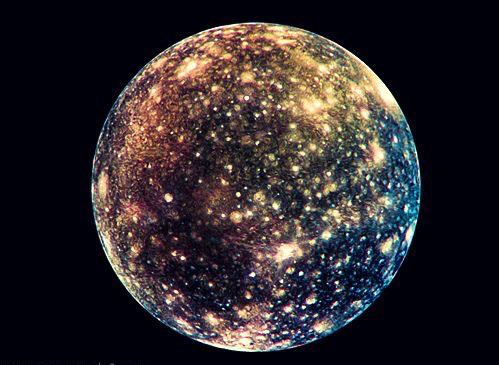
\includegraphics[width=.5\textwidth]{callisto.png}
\end{center}
\subsection{Saturn}
\begin{itemize}
    \item Less dense than water
    \item Also has many moons, such as Titan
\end{itemize}
\subsection{Uranus}
\begin{itemize}
    \item Only 4 times the size of Earth (much smaller than Jupiter or Saturn)
    \item Contains hydrogen compounds like water, ammonia, and methane, as well as hydrogen and helium gas
    \item Tipped almost perfectly on its side
\end{itemize}
\subsection{Neptune}
\begin{itemize}
    \item Mostly similar to Uranus, but larger and colder
    \item The moon Triton orbits Neptune ``backwards"
\end{itemize}
\subsection{Pluto}
\begin{itemize}
    \item Dwarf planet
    \item Eccentric orbit
    \item Here are pictures of the surface of Pluto:
\end{itemize}
\begin{center}
    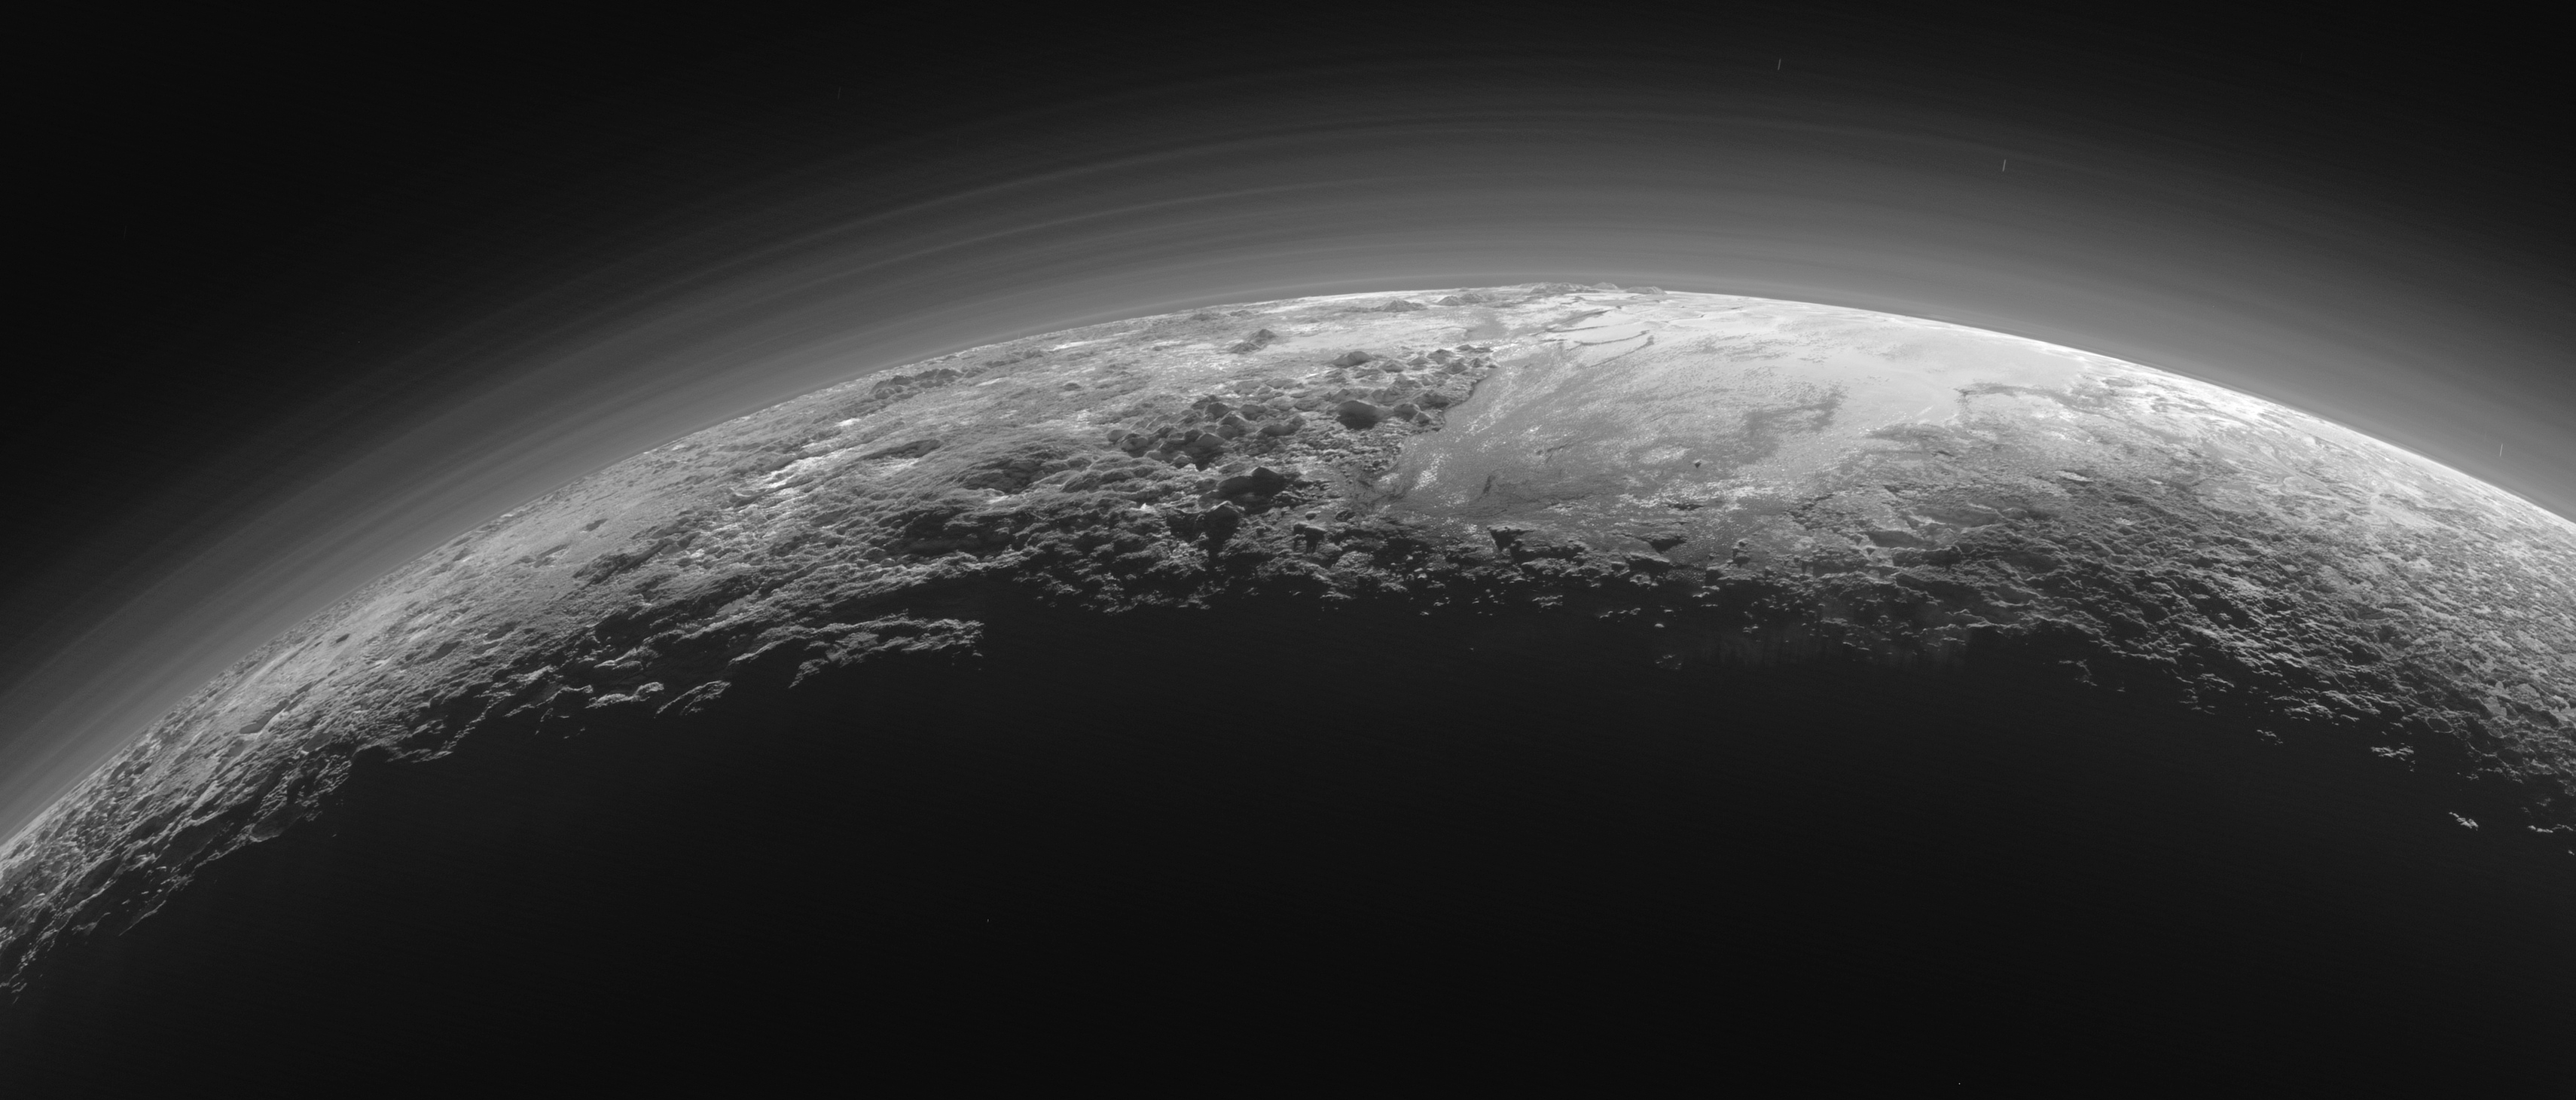
\includegraphics[width=\textwidth]{pluto surface.jpg}
\end{center}
\begin{center}
    \includegraphics[width=.5\textwidth]{sputnik planitia.jpg}
\end{center}
\subsection{Kuiper belt}
\begin{itemize}
    \item Extends from 30 to 50 AU from the sun
    \item Contains roughly 100,000 comets that are more than 100 km across
    \item Comets orbit in the same plane and direction as all the planets
\end{itemize}
\subsection{Oort cloud}
\begin{itemize}
    \item Extends out to 50,000 AU
    \item Contains about a trillion comets
    \item Do not orbit the sun in any orderly fashion
\end{itemize}
Note that Jovian planets often have rings, but terrestrial planets do not.
\par
``Nebular theory" explains the birth of the solar system.
\par
The ``frost line" is the circle around a star such that hydrogen compounds can freeze solid iff they are outside that circle. Most of the mass in a solar system is hydrogen and helium inside the frost line (and therefore fluid).
\par
Comets and asteroid are ``leftover planetesimals", formed by accretion in a solar nebula. Asteroids are rocky because they formed inside the frost line, and comets are icy because they formed outside the frost line. Accretion is easier when you can work with solids, which is why planets farther from a star tend to be larger -- they begin as solid planetesimals, which become massive enough to retain gas.
\par
Radioactive dating allows us to measure the age of a rock. For example, potassium-40 decays into argon-40 with a half life of 1.25 billion years, and since argon is inert, a rock won't contain argon when it is first formed, but potassium that decays into argon will remain trapped in the rock. Looking at the ration of potassium-40 to argon-40 can tell you how old that rock is. From this method, we see that the solar system is about 4.6 billion years old.
\par
Our theories of how the solar system form are not perfect, since they don't explain solar systems with ``hot Jupiters" -- gas giants which are closer tot heir star than Mercury is to the sun.

\end{document}
